%----------------------------------------------------------------------------------------
%	SPACEWEATHER EVENT.
%----------------------------------------------------------------------------------------
\section{Space weather event}
\begin{wrapfigure}[19]{r}{6.5cm}
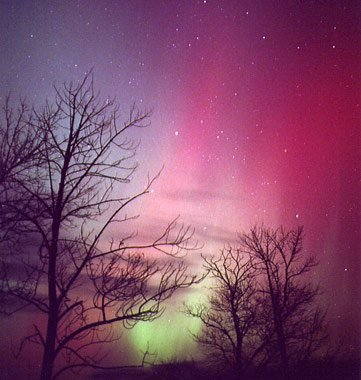
\includegraphics[width=6.5cm]{figures/SW_aurora_29oct_3.jpg}

\caption{Geomagnetic storm/ Aurora on the 29th of October \cite{spaceweather}.}
\label{fig:Aurora3}
\end{wrapfigure} 
In the rest of this document preprocessed data is used from the Halloween 2003 space weather event. This event took place from the 28th up to the 29th of October, with the main two peaks at 11:10 (28-10-2003) and 20:50 (29-10-2003) \cite{goes_x-ray_archive}. This solar weather event consisted of a series of solar flares and coronal mass ejections. The solar flare with the most energy was measured at 10:16:53 UCT. With an energy of $6.9\cdot10^{25}$\,Joule and a mass of $1.6 \cdot 10^{10}$\,gram \cite{CME_list}, one of the strongest ever measured by GOES.\\

Satellite-based systems and communications were affected, as well as the instruments onboard \cite{swpc-noaa}. Aircraft were advised to avoid high altitudes near the polar regions, and a one-hour-long power outage occurred in Sweden as a result of the solar activity. Auroras (figure \ref{fig:Aurora3}) were observed at latitudes as far south as Texas and the Mediterranean countries of Europe \cite{wiki_halloween_solar_stroms}.

\subsection{Solar flares}
\begin{wrapfigure}{r}{0.5\textwidth}
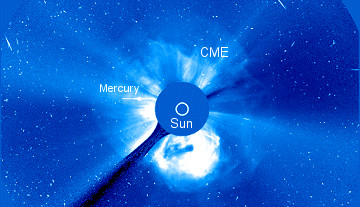
\includegraphics[width=.5\textwidth]{figures/SW_CME.jpg}

\caption{Solar image of a CME using a cronagraph\cite{spaceweather}.}
\label{fig:SW:CME}
\end{wrapfigure} 

On the 28th 12:18 UCT one of the most powerful solar flares in years erupted, this eruption, that caused a intense geomagnetic storm, is shown in figure \ref{fig:SW:CME}.The solar flares erupted out of 486 giant sunspots. It was measured X17  on the Richter scale of solar flares. This means that the peak had an energy above $7 \cdot 10^{-4}$\,W/m$^2$. It was also classified as a S3 storm, which means it has a flux of more than $10^3$ with $\geq$10\,MeV particles.  \cite{spaceweather}.\\


%----------------------------------------------------------------------------------------
%	GOES.
%----------------------------------------------------------------------------------------
\subsection{GOES}
In figure \ref{fig:goes_sem_data_oct} the space weather data from GOES10 (10th Geostationary Operational Environmental Satellite) over the month October is shown. In figure \ref{fig:goes_sem_data_nov} the data from the same satellite is shown over the month of November \cite{ngdc-noaa}. \\

WHAT IS SHOWN HERE!\\

DISCUSSION / INTERPRETATION

\begin{figure}[H]
\centering
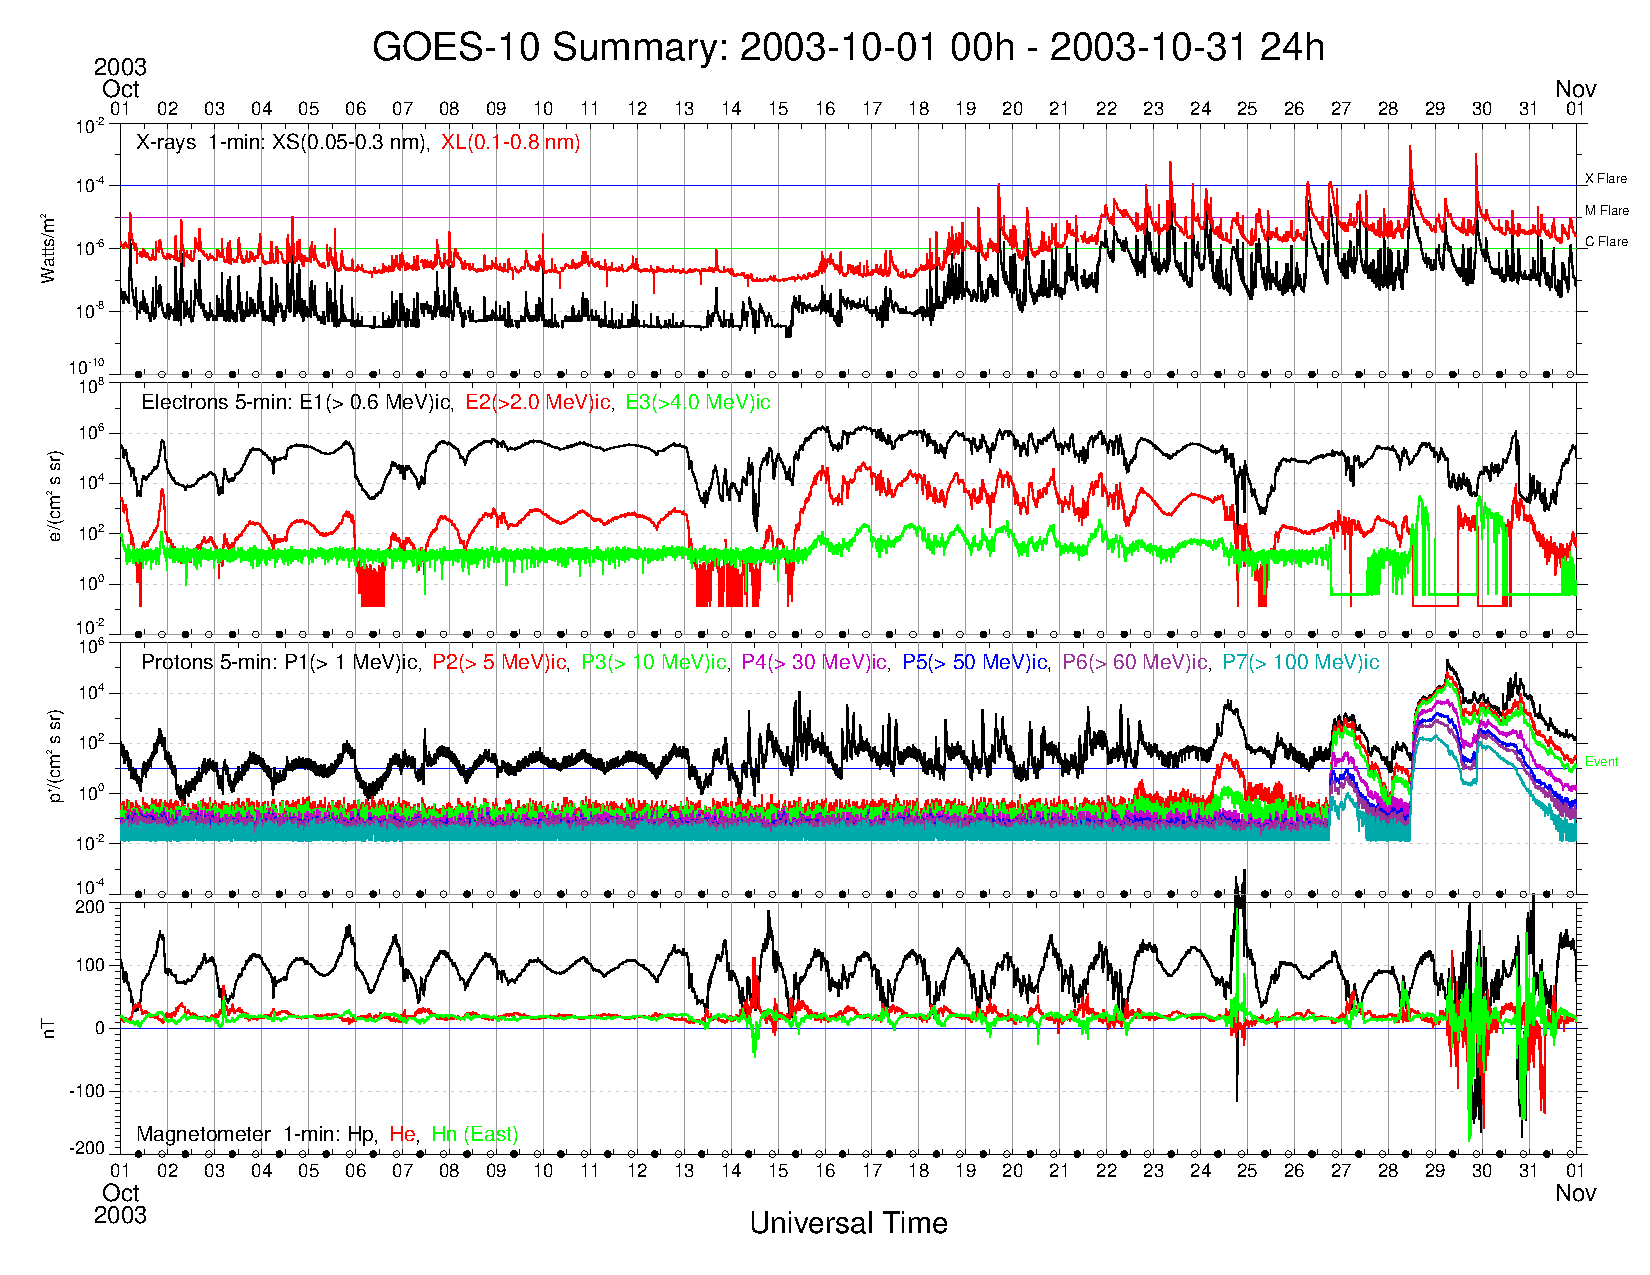
\includegraphics[page=1, width=.79\textwidth]{figures/goes10_oct.pdf}

\caption{\cite{ngdc-noaa}.}
\label{fig:goes_sem_data_oct}
\end{figure}

\begin{figure}[H]
\centering
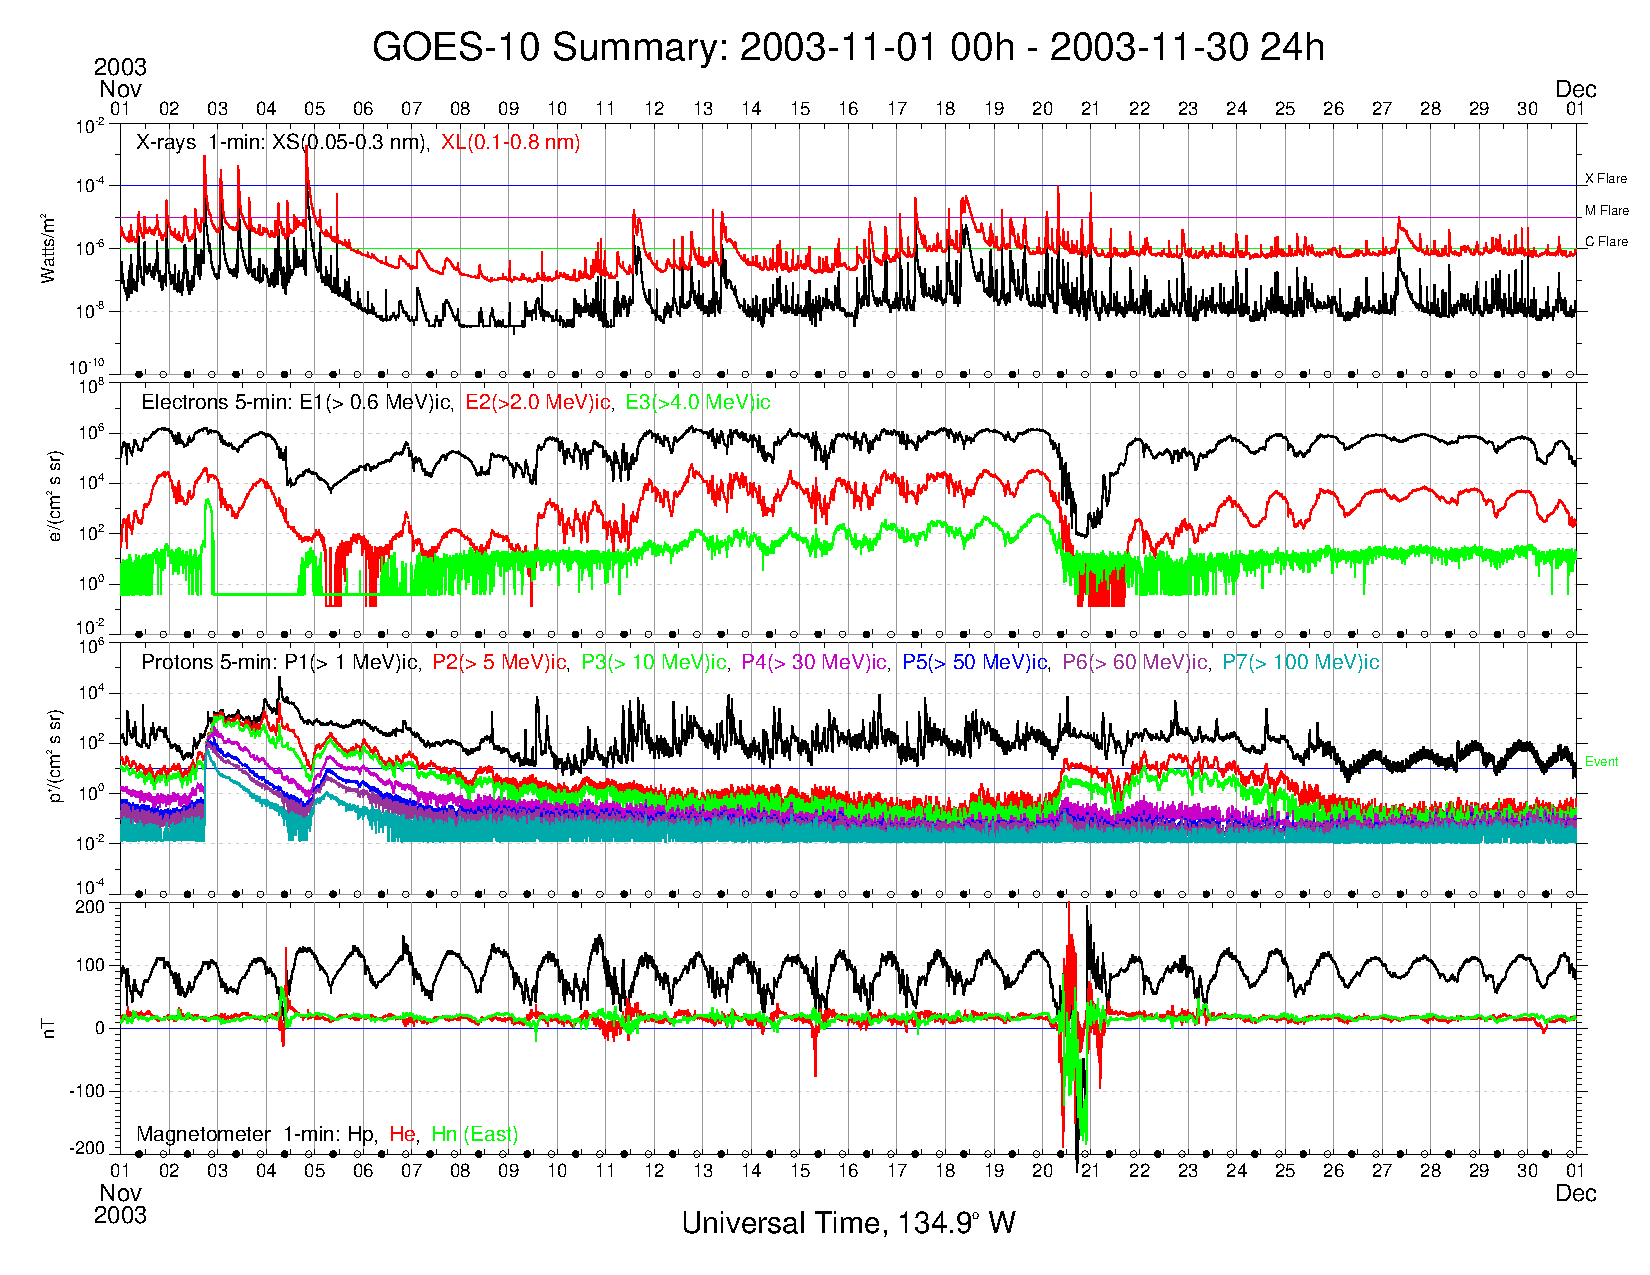
\includegraphics[page=1, width=.79\textwidth]{figures/goes10_nov.pdf}

\caption{\cite{ngdc-noaa}.}
\label{fig:goes_sem_data_nov}
\end{figure}


%----------------------------------------------------------------------------------------
%	IMAGE.
%----------------------------------------------------------------------------------------
\subsection{IMAGE}

text/ explanation

\begin{figure}[H]
        \begin{subfigure}[b]{0.33\textwidth}
                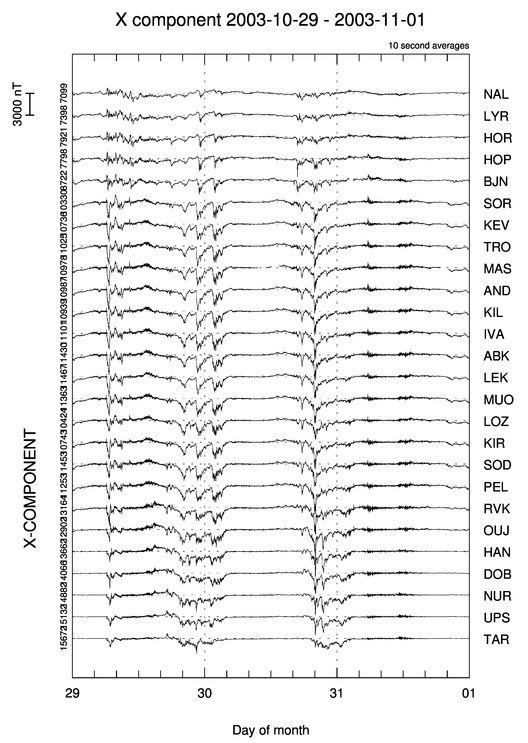
\includegraphics[width=\linewidth]{figures/IMAGE_X_gram.jpg}
                \caption{\cite{image}.}
				\label{fig:image_x_gram}
        \end{subfigure}%
        \begin{subfigure}[b]{0.34\textwidth}
                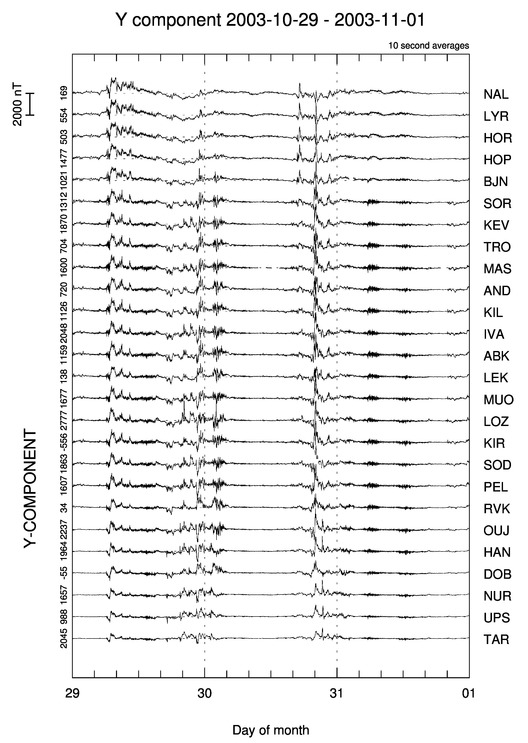
\includegraphics[width=\linewidth]{figures/IMAGE_Y_gram.jpg}
                \caption{\cite{image}.}
				\label{fig:image_y_gram}
        \end{subfigure}%
        \begin{subfigure}[b]{0.33\textwidth}
                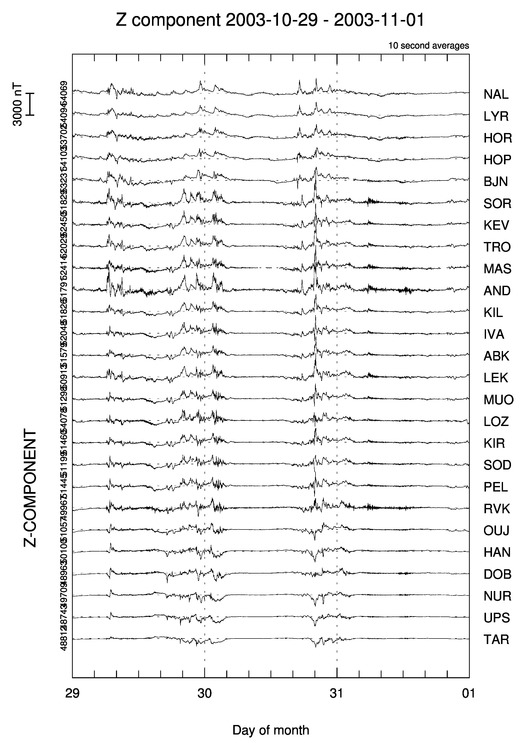
\includegraphics[width=\linewidth]{figures/IMAGE_Z_gram.jpg}
                \caption{\cite{image}.}
				\label{fig:image_z_gram}
        \end{subfigure}
        \caption{Pictures of animals}
        \label{fig:image_grams}
\end{figure}






sdfa






